% begin module limit-at-infinity-ex4
\begin{frame}
\begin{example} %[Example 4, p. 234]
Find the horizontal and vertical asymptotes of $f(x) = \frac{\sqrt{2x^2+1}}{3x-5}$.
\begin{columns}[c]
\column{.35\textwidth}
\psset{xunit=0.45cm, yunit=0.45cm}
\begin{pspicture}(-5, -5)(5.1,5.1) 
\psframe*[linecolor=white](-5,-5)(5.1,5.1) 
\psaxes[ticks=none, labels=none]{<->}(0,0)(-5,-5)(5,5)\tiny
\psLabels{5}{5}

\only<handout:0| 25->{ %
%Function formula: ((1+2 ((x)^{2}))^{1/2})/(-5+3 (x)) 
\psplot[linecolor=red, plotpoints=1000]{1.857}{5}{x 2 exp 2 mul 1 add 0.5 exp x 3 mul -5 add div } 
\psplot[linecolor=red, plotpoints=1000]{-5}{1.509}{x 2 exp 2 mul 1 add 0.5 exp x 3 mul -5 add div }
\rput[l](3,3){$y=f(x)$}
}

\only<handout:0| 24->{ %
\psline[linecolor=blue, linestyle=dashed](1.666666667,-4.95)(1.666666667,4.95)
\rput[l](1.7, -2.5){$x=\frac{5}{3}$}
}

\only<handout:0| 18->{ %
\psline[linecolor=blue, linestyle=dashed](-4.95,0.471404521)(4.95,0.471404521)
\rput[b](-3, 0.49){$\frac{\sqrt{2}}{3}$}
}
\only<handout:0| 22->{ %
\psline[linecolor=blue, linestyle=dashed](-4.95,-0.471404521)(4.95,-0.471404521)
\rput[t](-3, -0.49){$-\frac{\sqrt{2}}{3}$}
}
\end{pspicture} 
%\ \only<handout:0| -17>{%
%
\includegraphics[width=4.5cm]{curve-sketching/pictures/04-04-ex4a.pdf}%
%}%
%\only<handout:0| 18-21>{%
%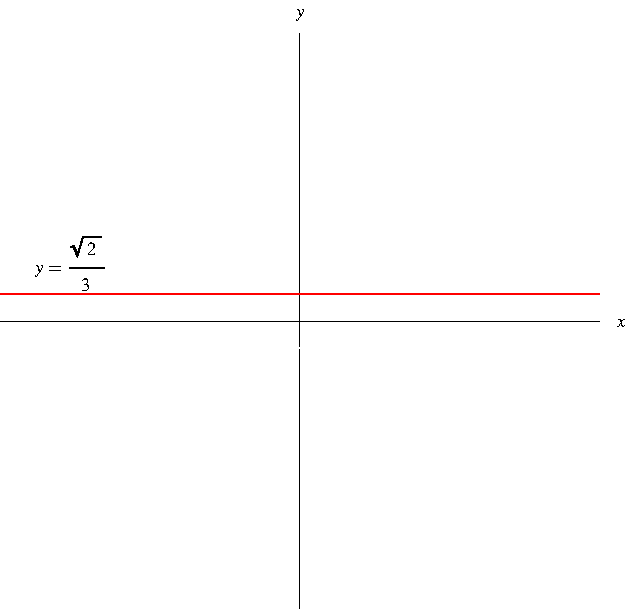
\includegraphics[width=4.5cm]{curve-sketching/pictures/04-04-ex4b.pdf}%
%}%
%\only<handout:0| 22-23>{%
%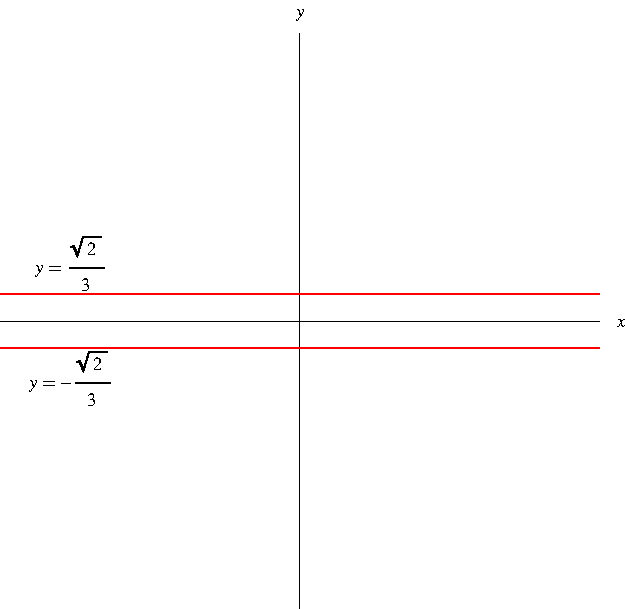
\includegraphics[width=4.5cm]{curve-sketching/pictures/04-04-ex4c.pdf}%
%}%
%\only<handout:0| 24>{%
%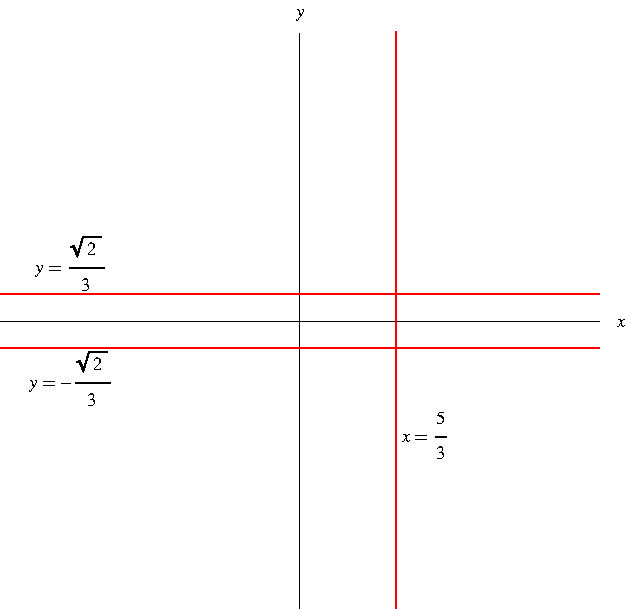
\includegraphics[width=4.5cm]{curve-sketching/pictures/04-04-ex4d.pdf}%
%}%
%\only<25->{%
%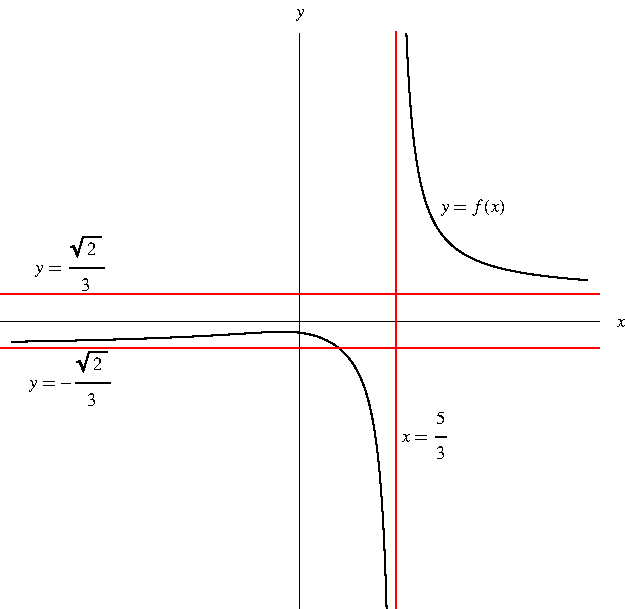
\includegraphics[width=4.5cm]{curve-sketching/pictures/04-04-ex4e.pdf}%
%}%
%\begin{itemize}

\uncover<4->{\alert<handout:0| 4>{If $x > 0$ then $x = \sqrt{x^2}$.}}

\uncover<20->{\alert<handout:0| 20>{If $x < 0$ then $x = -\sqrt{x^2}$.}}

\uncover<23->{\alert<handout:0| 23-24>{Vertical Asymptote: \uncover<24-25>{$x = \frac{5}{3}$.}}}
%\end{itemize}
\column{.65\textwidth}

\abovedisplayskip=0pt
\belowdisplayskip=0pt
\[
\begin{array}{l}
\uncover<2->{%
\displaystyle \lim_{x\to \infty} \frac{\sqrt{2x^2+1}}{3\alert<handout:0| 3>{x}-5}\uncover<3->{\alert<handout:0| 3>{\cdot \frac{\alert<handout:0| 4>{\frac{1}{x}}}{\frac{1}{x}}}}%
}%
%\\%
%& \uncover<4->{ = } &%
\uncover<4->{%
\displaystyle = \lim_{x\to \infty} \frac{\sqrt{\alert<handout:0| 5-6>{2x^2+1}}}{\alert<handout:0| 7-8>{3x-5}}\cdot \frac{\alert<handout:0| 4-6>{\frac{1}{\sqrt{x^2}}}}{\alert<handout:0| 7-8>{\frac{1}{x}}}%
}%
\\%
%& \uncover<8->{ = } &%
\uncover<5->{%
\displaystyle = \lim_{x\to \infty} \frac{\sqrt{\alert<handout:0| 5-6>{\uncover<6->{2+\frac{1}{x^2}}}}}{\alert<handout:0| 7-8>{\uncover<8->{3-\frac{5}{x}}}}%
}%
\uncover<9->{%
\displaystyle = \frac{\sqrt{\displaystyle \alert<handout:0| 10-11>{\lim_{x\to\infty}2} + \alert<handout:0| 12-13>{\lim_{x\to\infty}\frac{1}{x^2}}}}{\displaystyle \alert<handout:0| 14-15>{\lim_{x\to\infty}3} - \alert<handout:0| 16-17>{5\lim_{x\to\infty}\frac{1}{x}}}%
}%
\\%
%& \uncover<9->{ = } &%
\uncover<10->{%
\displaystyle = \frac{\sqrt{\uncover<11->{\alert<handout:0| 11>{2}} + \uncover<13->{\alert<handout:0| 13>{0}}}}{\uncover<15->{\alert<handout:0| 15>{3}} - \uncover<17->{\alert<handout:0| 17>{0}}}%
}%
\uncover<18->{%
 = \frac{\sqrt{2}}{3}%
}%
\end{array}
\]

\abovedisplayskip=0pt
\belowdisplayskip=0pt
\[
\begin{array}{l}
\uncover<2->{%
\displaystyle \lim_{x\to -\infty} \frac{\sqrt{2x^2+1}}{3\alert<handout:0| 19>{x}-5}\uncover<19->{\alert<handout:0| 19>{\cdot \frac{\alert<handout:0| 20>{\frac{1}{x}}}{\frac{1}{x}}}}%
}%
\uncover<20->{%
\displaystyle = \lim_{x\to -\infty} \frac{\sqrt{2x^2+1}}{3x-5}\cdot \frac{\alert<handout:0| 20>{\frac{-1}{\sqrt{x^2}}}}{\frac{1}{x}}%
}%
\\%
\uncover<21->{%
\displaystyle = \lim_{x\to -\infty} -\frac{\sqrt{2+\frac{1}{x^2}}}{3-\frac{5}{x}}%
}%
\uncover<22->{%
\displaystyle = -\frac{\sqrt{2}}{3}
}%
\end{array}
\]

\end{columns}
\end{example}
\end{frame}
% end module limit-at-infinity-ex4
